\documentclass[11pt]{article}
\usepackage[margin=1in]{geometry}
\usepackage{graphicx}
\usepackage{amsmath}
\usepackage{amssymb}
\usepackage{float}
\usepackage{subcaption}
\usepackage{booktabs}

\title{Regression Based Service Rate Estimation}

\begin{document}
\maketitle

\section{Overview}
  This week I worked on extending the regression model for service rate estimation to account for idleness.
  The main problem that we are trying to tackle is that the simple model, $\text{Days}_j = \beta_t \text{Trial}_j + \beta_p\text{Plea}_j +\epsilon_j$, doesn't account for idling judges. Hester's qualitative interviews with the judges indicates that harsher judges idle more often than more lenient judges.
  An overview of the results are below.

  \begin{itemize}
    \item \textbf{Iterative Idleness Estimation Using Expected Utilization:} This yields estimates of 3 days per trial, and about 14 pleas per day.

    \item \textbf{Iterative Idleness Estimation Taking Mins:} This yields estimates of 6.2 days per trial and 9.7 pleas per day.

    \item \textbf{Fixed Effects Model:} This yields estimates of 3.7 days per trial, and 10 pleas per day.
  \end{itemize}

  \begin{table}[H]
    \centering
    % \small
    \caption{Summary of Results}
    \begin{tabular}{llrr}
\toprule
      Model &         Group &  Pleas per Day &  Days per Trial \\
\midrule
        Min &        County &           6.92 &            4.41 \\
        Min &       Judge &           9.66 &            6.28 \\
        Min & Judge-County &          14.97 &            4.25 \\
  All time Min &        County &           7.12 &            3.65 \\
  All time Min &       Judge &           16.53 &            4.52 \\
  All time Min & Judge-County &          15.05 &            4.09 \\
Utilization &        County &           7.56 &            3.25 \\
Utilization &       Judge &          13.99 &            3.12 \\
Utilization & Judge-County &          20.90 &            1.73 \\
% Fixed Effects & Judge & 9.52 & 3.86 \\
% Fixed Effects & County & 10.99 & 4.34 \\
% Fixed Effects & Judge-County & 10.1 & 3.71 \\
\bottomrule
\end{tabular}

  \end{table}

\section{Iterative Idleness Estimation Using Expected Utilization}
  \textbf{Step 0:} We estimate the model, $\text{Days}_j = \beta_t\text{Trial}_j + \beta_p\text{Plea}_j +\epsilon_j$. \\

  \noindent \textbf{Steps 1-n:} We then use the estimates of $\beta^{(1)}_t$ and $\beta^{(1)}_p$ to estimate the expected number
  of days it would take each judge to complete their work. Mathematically: $\text{Expected Days}^{(1)}_j = \beta^{(1)}_p \cdot \text{Plea}_j + \beta^{(1)}_t \cdot \text{Trial}_j$. Then, the utilization for each judge would be: $\text{Utilization}^{(1)}_j = \frac{\text{Expected Days}^{(1)}_j}{\text{Days}_j}$. Let $\gamma^1 = \max_j \text{Utilization}^{(1)}_j$, be the maximum utilization amongst all judges. Each judges idleness will be: $\text{Idleness}^{(1)}_j = \frac{\text{Utilization}^{(1)}_j}{\gamma^{(1)}}$. We then set $\text{Days}^{(1)}_j = \text{Days}_j \cdot \text{Idleness}^{(1)}_j$. We then estimate the model $\text{Days}^{(1)}_j = \beta_t\text{Trial}_j + \beta_p\text{Plea}_j +\epsilon_j$ and repeat until convergence.

  \subsection{Judge Model}

    \begin{table}[H]
      \centering
      % \small
      \caption{Judge Model}
      \begin{center}
\begin{tabular}{lclc}
\toprule
\textbf{Dep. Variable:}    &        y         & \textbf{  R-squared (uncentered):}      &     1.000   \\
\textbf{Model:}            &       OLS        & \textbf{  Adj. R-squared (uncentered):} &     1.000   \\
\textbf{Method:}           &  Least Squares   & \textbf{  F-statistic:       }          & 4.033e+32   \\
\textbf{Date:}             & Wed, 08 Sep 2021 & \textbf{  Prob (F-statistic):}          &     0.00    \\
\textbf{Time:}             &     12:00:21     & \textbf{  Log-Likelihood:    }          &    1541.8   \\
\textbf{No. Observations:} &          50      & \textbf{  AIC:               }          &    -3080.   \\
\textbf{Df Residuals:}     &          48      & \textbf{  BIC:               }          &    -3076.   \\
\textbf{Df Model:}         &           2      & \textbf{                     }          &             \\
\bottomrule
\end{tabular}
\begin{tabular}{lcccccc}
               & \textbf{coef} & \textbf{std err} & \textbf{t} & \textbf{P$> |$t$|$} & \textbf{[0.025} & \textbf{0.975]}  \\
\midrule
\textbf{Plea}  &       0.0715  &     5.92e-18     &  1.21e+16  &         0.000        &        0.071    &        0.071     \\
\textbf{Trial} &       3.1154  &     3.49e-16     &  8.94e+15  &         0.000        &        3.115    &        3.115     \\
\bottomrule
\end{tabular}
\begin{tabular}{lclc}
\textbf{Omnibus:}       & 29.779 & \textbf{  Durbin-Watson:     } &    0.611  \\
\textbf{Prob(Omnibus):} &  0.000 & \textbf{  Jarque-Bera (JB):  } &   60.328  \\
\textbf{Skew:}          & -1.784 & \textbf{  Prob(JB):          } & 7.94e-14  \\
\textbf{Kurtosis:}      &  7.027 & \textbf{  Cond. No.          } &     85.5  \\
\bottomrule
\end{tabular}
%\caption{OLS Regression Results}
\end{center}

    \end{table}

    \begin{figure}[H]
      \centering
      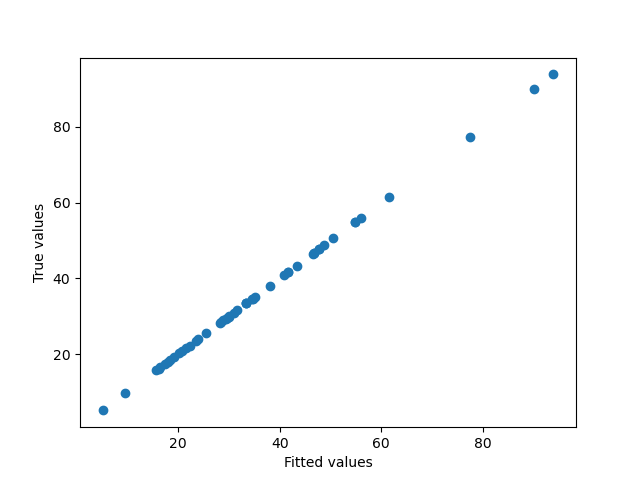
\includegraphics[width=0.65\textwidth]{../../../output/figures/Exploration/fit_utilization_JudgeID}
      \caption{True vs Fitted Values, Judge Model}
    \end{figure}

    \begin{table}[H]
      \centering
      % \small
      \caption{Judge Model}
      \begin{tabular}{rrr}
\toprule
 Iteration &  Beta P &  Beta T \\
\midrule
         0 &    0.15 &    6.48 \\
         1 &    0.07 &    3.12 \\
         2 &    0.07 &    3.12 \\
\bottomrule
\end{tabular}

    \end{table}

    \begin{table}[H]
      \centering
      \small
      \caption{Utilization at convergence, judge model}
      \begin{tabular}{lrrrrrrr}
\toprule
 JudgeID &  Plea &  Trial &   Days &  TrialDays &  PleaDays &  Utilization &  Idleness \\
\midrule
Judge 16 &  1041 &      5 &  90.00 &      15.58 &     74.42 &         1.00 &      1.00 \\
Judge 24 &   341 &     17 & 110.50 &      52.96 &     24.38 &         0.70 &      0.70 \\
Judge 42 &   283 &      3 &  44.00 &       9.35 &     20.23 &         0.67 &      0.67 \\
Judge 46 &   443 &      0 &  48.67 &       0.00 &     31.67 &         0.65 &      0.65 \\
 Judge 5 &   492 &      4 &  76.00 &      12.46 &     35.17 &         0.63 &      0.63 \\
 Judge 6 &   505 &      6 &  89.00 &      18.69 &     36.10 &         0.62 &      0.62 \\
Judge 39 &   389 &      6 &  76.00 &      18.69 &     27.81 &         0.61 &      0.61 \\
Judge 40 &   112 &      5 &  40.00 &      15.58 &      8.01 &         0.59 &      0.59 \\
 Judge 7 &   572 &     17 & 167.00 &      52.96 &     40.89 &         0.56 &      0.56 \\
Judge 11 &   244 &     12 & 107.00 &      37.38 &     17.44 &         0.51 &      0.51 \\
Judge 33 &   479 &      4 &  98.00 &      12.46 &     34.24 &         0.48 &      0.48 \\
Judge 50 &   469 &      9 & 129.50 &      28.04 &     33.53 &         0.48 &      0.48 \\
Judge 22 &   480 &      4 &  98.50 &      12.46 &     34.32 &         0.47 &      0.47 \\
Judge 38 &   247 &      4 &  64.00 &      12.46 &     17.66 &         0.47 &      0.47 \\
Judge 25 &   527 &      1 &  87.00 &       3.12 &     37.68 &         0.47 &      0.47 \\
Judge 10 &   315 &      9 & 108.50 &      28.04 &     22.52 &         0.47 &      0.47 \\
Judge 26 &   450 &      5 & 103.00 &      15.58 &     32.17 &         0.46 &      0.46 \\
 Judge 2 &   390 &      9 & 121.00 &      28.04 &     27.88 &         0.46 &      0.46 \\
Judge 44 &   395 &      2 &  78.00 &       6.23 &     28.24 &         0.44 &      0.44 \\
Judge 47 &   388 &      5 & 100.00 &      15.58 &     27.74 &         0.43 &      0.43 \\
Judge 30 &   147 &     10 &  96.50 &      31.15 &     10.51 &         0.43 &      0.43 \\
 Judge 8 &   215 &      5 &  72.00 &      15.58 &     15.37 &         0.43 &      0.43 \\
Judge 17 &   288 &      3 &  73.00 &       9.35 &     20.59 &         0.41 &      0.41 \\
 Judge 3 &   193 &      5 &  72.00 &      15.58 &     13.80 &         0.41 &      0.41 \\
Judge 27 &   204 &      3 &  60.00 &       9.35 &     14.58 &         0.40 &      0.40 \\
Judge 32 &   226 &      3 &  64.00 &       9.35 &     16.16 &         0.40 &      0.40 \\
Judge 18 &   202 &     11 & 123.00 &      34.27 &     14.44 &         0.40 &      0.40 \\
 Judge 4 &   162 &      7 &  85.50 &      21.81 &     11.58 &         0.39 &      0.39 \\
Judge 19 &   404 &      2 &  92.00 &       6.23 &     28.88 &         0.38 &      0.38 \\
Judge 34 &   355 &      1 &  75.00 &       3.12 &     25.38 &         0.38 &      0.38 \\
Judge 37 &   112 &      3 &  46.50 &       9.35 &      8.01 &         0.37 &      0.37 \\
Judge 13 &   228 &      7 & 105.50 &      21.81 &     16.30 &         0.36 &      0.36 \\
Judge 48 &   317 &      2 &  80.00 &       6.23 &     22.66 &         0.36 &      0.36 \\
Judge 29 &   293 &      4 &  98.50 &      12.46 &     20.95 &         0.34 &      0.34 \\
Judge 36 &   139 &      2 &  49.00 &       6.23 &      9.94 &         0.33 &      0.33 \\
 Judge 9 &   398 &      2 & 105.50 &       6.23 &     28.45 &         0.33 &      0.33 \\
Judge 31 &   171 &      2 &  58.00 &       6.23 &     12.23 &         0.32 &      0.32 \\
Judge 15 &   144 &      2 &  52.00 &       6.23 &     10.29 &         0.32 &      0.32 \\
Judge 21 &   170 &      3 &  70.00 &       9.35 &     12.15 &         0.31 &      0.31 \\
Judge 49 &   321 &      6 & 137.00 &      18.69 &     22.95 &         0.30 &      0.30 \\
Judge 23 &   139 &      3 &  64.00 &       9.35 &      9.94 &         0.30 &      0.30 \\
Judge 28 &   353 &      1 &  97.00 &       3.12 &     25.24 &         0.29 &      0.29 \\
Judge 35 &   176 &      1 &  54.00 &       3.12 &     12.58 &         0.29 &      0.29 \\
Judge 43 &   283 &      0 &  72.00 &       0.00 &     20.23 &         0.28 &      0.28 \\
 Judge 1 &   293 &      4 & 122.00 &      12.46 &     20.95 &         0.27 &      0.27 \\
Judge 12 &   268 &      1 &  82.00 &       3.12 &     19.16 &         0.27 &      0.27 \\
Judge 14 &   208 &      1 &  68.00 &       3.12 &     14.87 &         0.26 &      0.26 \\
Judge 41 &    91 &      1 &  38.00 &       3.12 &      6.51 &         0.25 &      0.25 \\
Judge 45 &   161 &      3 &  90.00 &       9.35 &     11.51 &         0.23 &      0.23 \\
Judge 20 &    72 &      0 &  23.00 &       0.00 &      5.15 &         0.22 &      0.22 \\
\bottomrule
\end{tabular}

    \end{table}

  \subsection{County Model}

    \begin{table}[H]
      \centering
      % \small
      \caption{County Model}
      \begin{center}
\begin{tabular}{lclc}
\toprule
\textbf{Dep. Variable:}    &        y         & \textbf{  R-squared (uncentered):}      &     1.000   \\
\textbf{Model:}            &       OLS        & \textbf{  Adj. R-squared (uncentered):} &     1.000   \\
\textbf{Method:}           &  Least Squares   & \textbf{  F-statistic:       }          & 1.261e+33   \\
\textbf{Date:}             & Wed, 08 Sep 2021 & \textbf{  Prob (F-statistic):}          &     0.00    \\
\textbf{Time:}             &     12:00:22     & \textbf{  Log-Likelihood:    }          &    1409.1   \\
\textbf{No. Observations:} &          46      & \textbf{  AIC:               }          &    -2814.   \\
\textbf{Df Residuals:}     &          44      & \textbf{  BIC:               }          &    -2810.   \\
\textbf{Df Model:}         &           2      & \textbf{                     }          &             \\
\bottomrule
\end{tabular}
\begin{tabular}{lcccccc}
               & \textbf{coef} & \textbf{std err} & \textbf{t} & \textbf{P$> |$t$|$} & \textbf{[0.025} & \textbf{0.975]}  \\
\midrule
\textbf{Plea}  &       0.1324  &      8.1e-18     &  1.63e+16  &         0.000        &        0.132    &        0.132     \\
\textbf{Trial} &       3.2526  &      5.3e-16     &  6.14e+15  &         0.000        &        3.253    &        3.253     \\
\bottomrule
\end{tabular}
\begin{tabular}{lclc}
\textbf{Omnibus:}       & 36.252 & \textbf{  Durbin-Watson:     } &    1.962  \\
\textbf{Prob(Omnibus):} &  0.000 & \textbf{  Jarque-Bera (JB):  } &  192.576  \\
\textbf{Skew:}          & -1.678 & \textbf{  Prob(JB):          } & 1.52e-42  \\
\textbf{Kurtosis:}      & 12.445 & \textbf{  Cond. No.          } &     149.  \\
\bottomrule
\end{tabular}
%\caption{OLS Regression Results}
\end{center}

    \end{table}

    \begin{figure}[H]
      \centering
      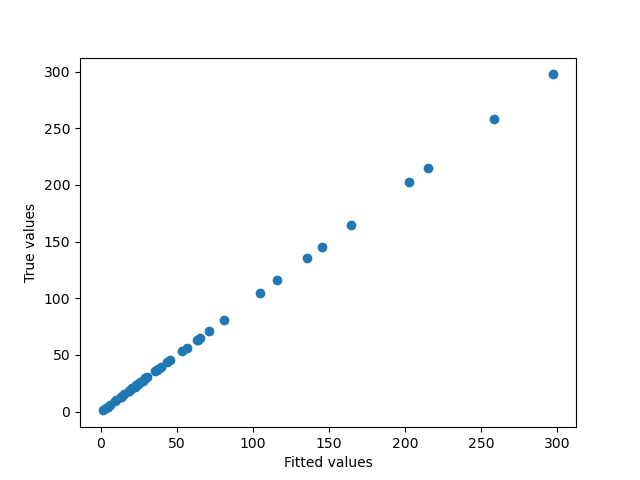
\includegraphics[width=0.65\textwidth]{../../../output/figures/Exploration/fit_utilization_County}
      \caption{True vs Fitted Values, Judge-County Model}
    \end{figure}

    \begin{table}[H]
      \centering
      % \small
      \caption{Judge Model}
      \begin{tabular}{rrr}
\toprule
 Iteration &  Beta P &  Beta T \\
\midrule
         0 &    0.17 &    4.23 \\
         1 &    0.13 &    3.25 \\
         2 &    0.13 &    3.25 \\
\bottomrule
\end{tabular}

    \end{table}

    \begin{table}[H]
      \centering
      \small
      \caption{Utilization at convergence, county model}
      \begin{tabular}{lrrrrrrr}
\toprule
      County &  Plea &  Trial &   Days &  TrialDays &  PleaDays &  Utilization &  Idleness \\
\midrule
 Spartanburg &  1063 &     19 & 202.50 &      61.80 &    140.70 &         1.00 &      1.00 \\
  Greenville &  1608 &     14 & 272.00 &      45.54 &    212.84 &         0.95 &      0.95 \\
  Dorchester &   291 &     10 &  78.00 &      32.53 &     38.52 &         0.91 &      0.91 \\
    Anderson &   655 &     15 & 161.00 &      48.79 &     86.70 &         0.84 &      0.84 \\
      Oconee &   230 &      2 &  46.50 &       6.51 &     30.44 &         0.79 &      0.79 \\
    Florence &   754 &      5 & 146.50 &      16.26 &     99.80 &         0.79 &      0.79 \\
       Aiken &   343 &     11 & 105.50 &      35.78 &     45.40 &         0.77 &      0.77 \\
    Berkeley &   382 &      4 &  83.00 &      13.01 &     50.56 &         0.77 &      0.77 \\
        York &   777 &     19 & 216.50 &      61.80 &    102.85 &         0.76 &      0.76 \\
   Lexington &   644 &      6 & 141.00 &      19.52 &     85.24 &         0.74 &      0.74 \\
  Charleston &  1329 &     12 & 291.50 &      39.03 &    175.91 &         0.74 &      0.74 \\
    Barnwell &   113 &      1 &  25.00 &       3.25 &     14.96 &         0.73 &      0.73 \\
       Horry &   655 &     18 & 199.50 &      58.55 &     86.70 &         0.73 &      0.73 \\
   Greenwood &   370 &      5 &  90.00 &      16.26 &     48.97 &         0.72 &      0.72 \\
    Richland &  1633 &     25 & 417.00 &      81.31 &    216.15 &         0.71 &      0.71 \\
    Cherokee &   128 &      7 &  57.50 &      22.77 &     16.94 &         0.69 &      0.69 \\
  Georgetown &   230 &      7 &  79.00 &      22.77 &     30.44 &         0.67 &      0.67 \\
      Sumter &   353 &      5 & 100.00 &      16.26 &     46.72 &         0.63 &      0.63 \\
     Pickens &   254 &      3 &  73.00 &       9.76 &     33.62 &         0.59 &      0.59 \\
     Laurens &   293 &      2 &  82.00 &       6.51 &     38.78 &         0.55 &      0.55 \\
  Orangeburg &   327 &      4 & 104.00 &      13.01 &     43.28 &         0.54 &      0.54 \\
      Saluda &    74 &      1 &  25.00 &       3.25 &      9.79 &         0.52 &      0.52 \\
     Kershaw &   268 &      0 &  68.00 &       0.00 &     35.47 &         0.52 &      0.52 \\
      Jasper &    73 &      1 &  25.00 &       3.25 &      9.66 &         0.52 &      0.52 \\
Chesterfield &   131 &      4 &  59.00 &      13.01 &     17.34 &         0.51 &      0.51 \\
      Marion &   171 &      1 &  51.00 &       3.25 &     22.63 &         0.51 &      0.51 \\
       Union &   147 &      3 &  59.00 &       9.76 &     19.46 &         0.50 &      0.50 \\
   Abbeville &   118 &      2 &  45.00 &       6.51 &     15.62 &         0.49 &      0.49 \\
   Fairfield &    62 &      5 &  50.00 &      16.26 &      8.21 &         0.49 &      0.49 \\
    Newberry &   149 &      1 &  48.00 &       3.25 &     19.72 &         0.48 &      0.48 \\
         Lee &    91 &      2 &  40.50 &       6.51 &     12.04 &         0.46 &      0.46 \\
   Edgefield &   116 &      0 &  34.00 &       0.00 &     15.35 &         0.45 &      0.45 \\
   Clarendon &   158 &      2 &  63.50 &       6.51 &     20.91 &         0.43 &      0.43 \\
  Darlington &   172 &      2 &  68.00 &       6.51 &     22.77 &         0.43 &      0.43 \\
     Bamberg &    70 &      0 &  22.67 &       0.00 &      9.27 &         0.41 &      0.41 \\
    Colleton &   124 &      1 &  50.50 &       3.25 &     16.41 &         0.39 &      0.39 \\
   Lancaster &   158 &      1 &  67.00 &       3.25 &     20.91 &         0.36 &      0.36 \\
    Marlboro &   174 &      0 &  66.50 &       0.00 &     23.03 &         0.35 &      0.35 \\
    Beaufort &   183 &      4 & 109.00 &      13.01 &     24.22 &         0.34 &      0.34 \\
Williamsburg &   156 &      0 &  61.00 &       0.00 &     20.65 &         0.34 &      0.34 \\
   McCormick &    47 &      0 &  23.00 &       0.00 &      6.22 &         0.27 &      0.27 \\
     Calhoun &    27 &      0 &  14.00 &       0.00 &      3.57 &         0.26 &      0.26 \\
     Chester &    79 &      1 &  59.00 &       3.25 &     10.46 &         0.23 &      0.23 \\
     Hampton &    33 &      0 &  19.00 &       0.00 &      4.37 &         0.23 &      0.23 \\
      Dillon &    74 &      0 &  48.00 &       0.00 &      9.79 &         0.20 &      0.20 \\
   Allendale &     8 &      0 &  14.00 &       0.00 &      1.06 &         0.08 &      0.08 \\
\bottomrule
\end{tabular}

    \end{table}

  \subsection{Judge-County Model}

    \begin{table}[H]
      \centering
      % \small
      \caption{County Model}
      \begin{center}
\begin{tabular}{lclc}
\toprule
\textbf{Dep. Variable:}    &        y         & \textbf{  R-squared (uncentered):}      &     1.000   \\
\textbf{Model:}            &       OLS        & \textbf{  Adj. R-squared (uncentered):} &     1.000   \\
\textbf{Method:}           &  Least Squares   & \textbf{  F-statistic:       }          & 1.306e+33   \\
\textbf{Date:}             & Wed, 08 Sep 2021 & \textbf{  Prob (F-statistic):}          &     0.00    \\
\textbf{Time:}             &     12:00:22     & \textbf{  Log-Likelihood:    }          &    8998.6   \\
\textbf{No. Observations:} &         278      & \textbf{  AIC:               }          & -1.799e+04  \\
\textbf{Df Residuals:}     &         276      & \textbf{  BIC:               }          & -1.799e+04  \\
\textbf{Df Model:}         &           2      & \textbf{                     }          &             \\
\bottomrule
\end{tabular}
\begin{tabular}{lcccccc}
               & \textbf{coef} & \textbf{std err} & \textbf{t} & \textbf{P$> |$t$|$} & \textbf{[0.025} & \textbf{0.975]}  \\
\midrule
\textbf{Plea}  &       0.0478  &     1.72e-18     &  2.79e+16  &         0.000        &        0.048    &        0.048     \\
\textbf{Trial} &       1.7321  &      8.7e-17     &  1.99e+16  &         0.000        &        1.732    &        1.732     \\
\bottomrule
\end{tabular}
\begin{tabular}{lclc}
\textbf{Omnibus:}       & 127.483 & \textbf{  Durbin-Watson:     } &    1.817  \\
\textbf{Prob(Omnibus):} &   0.000 & \textbf{  Jarque-Bera (JB):  } & 1614.656  \\
\textbf{Skew:}          &  -1.487 & \textbf{  Prob(JB):          } &     0.00  \\
\textbf{Kurtosis:}      &  14.426 & \textbf{  Cond. No.          } &     61.2  \\
\bottomrule
\end{tabular}
%\caption{OLS Regression Results}
\end{center}

    \end{table}

    \begin{figure}[H]
      \centering
      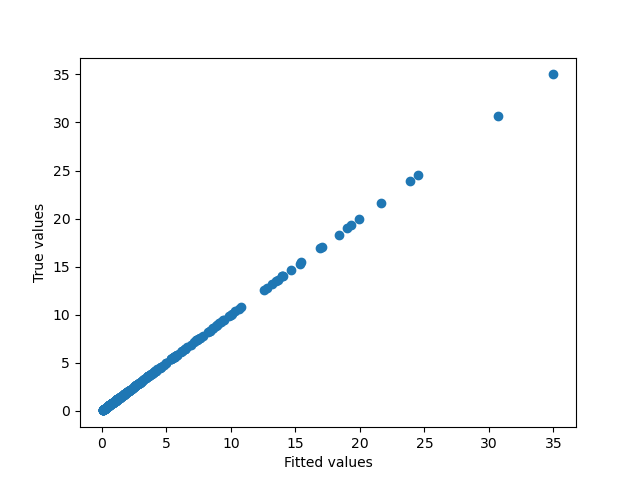
\includegraphics[width=0.65\textwidth]{../../../output/figures/Exploration/fit_utilization_JudgeIDCounty}
      \caption{True vs Fitted Values, Judge-County Model}
    \end{figure}

    \begin{table}[H]
      \centering
      % \small
      \caption{Judge-County Model}
      \begin{tabular}{rrr}
\toprule
 Iteration &  Beta P &  Beta T \\
\midrule
         0 &    0.13 &    4.76 \\
         1 &    0.05 &    1.73 \\
         2 &    0.05 &    1.73 \\
\bottomrule
\end{tabular}

    \end{table}

    \begin{table}[H]
      \centering
      \small
      \caption{Utilization at convergence, judge-county model}
      \begin{tabular}{llrrrrrrr}
\toprule
 JudgeID &       County &  Plea &  Trial &  Days &  TrialDays &  PleaDays &  Utilization &  Idleness \\
\midrule
Judge 16 &  Spartanburg &   623 &      3 & 35.00 &       5.20 &     29.80 &         1.00 &      1.00 \\
 Judge 8 &        Aiken &    36 &      1 &  4.00 &       1.73 &      1.72 &         0.86 &      0.86 \\
Judge 16 &   Greenville &   307 &      0 & 21.00 &       0.00 &     14.69 &         0.70 &      0.70 \\
Judge 42 &       Oconee &    35 &      1 &  5.00 &       1.73 &      1.67 &         0.68 &      0.68 \\
Judge 16 &        Aiken &    12 &      1 &  4.00 &       1.73 &      0.57 &         0.58 &      0.58 \\
Judge 25 &    Lexington &    23 &      1 &  5.00 &       1.73 &      1.10 &         0.57 &      0.57 \\
 Judge 8 &     Beaufort &     9 &      3 & 10.00 &       5.20 &      0.43 &         0.56 &      0.56 \\
Judge 46 &   Charleston &   222 &      0 & 19.00 &       0.00 &     10.62 &         0.56 &      0.56 \\
Judge 47 &   Georgetown &    66 &      3 & 15.00 &       5.20 &      3.16 &         0.56 &      0.56 \\
Judge 46 &      Bamberg &    19 &      0 &  1.67 &       0.00 &      0.91 &         0.55 &      0.55 \\
 Judge 7 &   Dorchester &   187 &      9 & 45.00 &      15.59 &      8.95 &         0.55 &      0.55 \\
Judge 38 &     Berkeley &    40 &      2 & 10.00 &       3.46 &      1.91 &         0.54 &      0.54 \\
Judge 46 &        Horry &    53 &      0 &  5.00 &       0.00 &      2.54 &         0.51 &      0.51 \\
Judge 25 &   Greenville &   210 &      0 & 20.00 &       0.00 &     10.05 &         0.50 &      0.50 \\
Judge 35 &     Colleton &    16 &      1 &  5.00 &       1.73 &      0.77 &         0.50 &      0.50 \\
Judge 24 &         York &   207 &     12 & 62.50 &      20.79 &      9.90 &         0.49 &      0.49 \\
 Judge 5 &        Horry &   189 &      1 & 22.00 &       1.73 &      9.04 &         0.49 &      0.49 \\
Judge 19 &         York &   153 &      0 & 15.00 &       0.00 &      7.32 &         0.49 &      0.49 \\
Judge 26 &     Anderson &   252 &      4 & 39.00 &       6.93 &     12.06 &         0.49 &      0.49 \\
Judge 38 &       Sumter &     4 &      1 &  4.00 &       1.73 &      0.19 &         0.48 &      0.48 \\
Judge 28 &     Richland &   102 &      1 & 14.00 &       1.73 &      4.88 &         0.47 &      0.47 \\
 Judge 6 &     Florence &   285 &      0 & 29.00 &       0.00 &     13.63 &         0.47 &      0.47 \\
Judge 15 &   Orangeburg &     3 &      1 &  4.00 &       1.73 &      0.14 &         0.47 &      0.47 \\
Judge 10 &    Greenwood &    24 &      2 & 10.00 &       3.46 &      1.15 &         0.46 &      0.46 \\
Judge 42 &      Pickens &    58 &      1 & 10.00 &       1.73 &      2.77 &         0.45 &      0.45 \\
Judge 18 &        Horry &   103 &      6 & 34.00 &      10.39 &      4.93 &         0.45 &      0.45 \\
Judge 10 &         York &     1 &      1 &  4.00 &       1.73 &      0.05 &         0.44 &      0.44 \\
Judge 37 &    Clarendon &    10 &      1 &  5.00 &       1.73 &      0.48 &         0.44 &      0.44 \\
 Judge 5 &     Richland &   245 &      3 & 39.00 &       5.20 &     11.72 &         0.43 &      0.43 \\
Judge 50 &     Richland &   163 &      8 & 50.00 &      13.86 &      7.80 &         0.43 &      0.43 \\
Judge 42 &   Greenville &   180 &      1 & 24.00 &       1.73 &      8.61 &         0.43 &      0.43 \\
Judge 24 &     Cherokee &    44 &      2 & 13.00 &       3.46 &      2.10 &         0.43 &      0.43 \\
Judge 43 &   Charleston &    67 &      0 &  7.50 &       0.00 &      3.21 &         0.43 &      0.43 \\
Judge 17 &   Greenville &   142 &      1 & 20.00 &       1.73 &      6.79 &         0.43 &      0.43 \\
Judge 41 &     Berkeley &     8 &      1 &  5.00 &       1.73 &      0.38 &         0.42 &      0.42 \\
Judge 46 &  Spartanburg &    44 &      0 &  5.00 &       0.00 &      2.10 &         0.42 &      0.42 \\
Judge 44 &   Greenville &   209 &      0 & 24.00 &       0.00 &     10.00 &         0.42 &      0.42 \\
Judge 46 &    Lexington &    87 &      0 & 10.00 &       0.00 &      4.16 &         0.42 &      0.42 \\
Judge 39 &       Oconee &     7 &      1 &  5.00 &       1.73 &      0.33 &         0.41 &      0.41 \\
Judge 33 &   Darlington &     7 &      1 &  5.00 &       1.73 &      0.33 &         0.41 &      0.41 \\
Judge 39 &     Anderson &   203 &      2 & 32.00 &       3.46 &      9.71 &         0.41 &      0.41 \\
Judge 19 &    Lexington &    43 &      0 &  5.00 &       0.00 &      2.06 &         0.41 &      0.41 \\
Judge 19 &       Sumter &    41 &      1 &  9.00 &       1.73 &      1.96 &         0.41 &      0.41 \\
Judge 26 &    Lexington &    17 &      0 &  2.00 &       0.00 &      0.81 &         0.41 &      0.41 \\
Judge 39 &     Barnwell &    17 &      0 &  2.00 &       0.00 &      0.81 &         0.41 &      0.41 \\
Judge 39 &    Lexington &   113 &      2 & 22.00 &       3.46 &      5.41 &         0.40 &      0.40 \\
Judge 26 &    Greenwood &    31 &      1 &  8.00 &       1.73 &      1.48 &         0.40 &      0.40 \\
Judge 16 &      Pickens &    41 &      0 &  5.00 &       0.00 &      1.96 &         0.39 &      0.39 \\
Judge 21 &   Charleston &    50 &      2 & 15.00 &       3.46 &      2.39 &         0.39 &      0.39 \\
 Judge 3 &   Charleston &    82 &      2 & 19.00 &       3.46 &      3.92 &         0.39 &      0.39 \\
Judge 15 &   Charleston &     4 &      1 &  5.00 &       1.73 &      0.19 &         0.38 &      0.38 \\
 Judge 9 & Chesterfield &     8 &      0 &  1.00 &       0.00 &      0.38 &         0.38 &      0.38 \\
 Judge 4 &    Fairfield &     7 &      2 & 10.00 &       3.46 &      0.33 &         0.38 &      0.38 \\
 Judge 6 &        Horry &   140 &      6 & 45.00 &      10.39 &      6.70 &         0.38 &      0.38 \\
Judge 22 &   Greenville &   311 &      2 & 49.00 &       3.46 &     14.88 &         0.37 &      0.37 \\
Judge 30 &     Anderson &    75 &      6 & 38.00 &      10.39 &      3.59 &         0.37 &      0.37 \\
Judge 24 &        Union &    40 &      1 & 10.00 &       1.73 &      1.91 &         0.36 &      0.36 \\
 Judge 2 &        Aiken &   199 &      6 & 55.00 &      10.39 &      9.52 &         0.36 &      0.36 \\
Judge 39 &       Saluda &    39 &      1 & 10.00 &       1.73 &      1.87 &         0.36 &      0.36 \\
Judge 10 &  Spartanburg &    44 &      2 & 15.50 &       3.46 &      2.10 &         0.36 &      0.36 \\
Judge 48 &   Greenville &    75 &      0 & 10.00 &       0.00 &      3.59 &         0.36 &      0.36 \\
 Judge 3 &        Horry &    40 &      2 & 15.00 &       3.46 &      1.91 &         0.36 &      0.36 \\
 Judge 7 &   Charleston &    81 &      5 & 35.00 &       8.66 &      3.87 &         0.36 &      0.36 \\
Judge 44 &    Greenwood &   107 &      2 & 24.00 &       3.46 &      5.12 &         0.36 &      0.36 \\
Judge 16 &     Anderson &    37 &      0 &  5.00 &       0.00 &      1.77 &         0.35 &      0.35 \\
Judge 48 &  Spartanburg &    37 &      0 &  5.00 &       0.00 &      1.77 &         0.35 &      0.35 \\
Judge 40 &   Greenville &   112 &      5 & 40.00 &       8.66 &      5.36 &         0.35 &      0.35 \\
 Judge 8 &   Dorchester &    37 &      1 & 10.00 &       1.73 &      1.77 &         0.35 &      0.35 \\
Judge 16 &     Cherokee &     0 &      1 &  5.00 &       1.73 &      0.00 &         0.35 &      0.35 \\
Judge 32 &   Charleston &   123 &      1 & 22.00 &       1.73 &      5.88 &         0.35 &      0.35 \\
Judge 10 &      Laurens &   134 &      2 & 29.00 &       3.46 &      6.41 &         0.34 &      0.34 \\
Judge 43 &     Berkeley &   135 &      0 & 19.00 &       0.00 &      6.46 &         0.34 &      0.34 \\
Judge 45 & Williamsburg &     7 &      0 &  1.00 &       0.00 &      0.33 &         0.33 &      0.33 \\
Judge 34 &     Richland &   130 &      0 & 19.00 &       0.00 &      6.22 &         0.33 &      0.33 \\
Judge 33 &     Richland &   367 &      1 & 59.00 &       1.73 &     17.56 &         0.33 &      0.33 \\
Judge 11 &  Spartanburg &   173 &      9 & 73.00 &      15.59 &      8.28 &         0.33 &      0.33 \\
Judge 18 & Chesterfield &    21 &      3 & 19.00 &       5.20 &      1.00 &         0.33 &      0.33 \\
 Judge 2 &     Barnwell &    64 &      1 & 15.00 &       1.73 &      3.06 &         0.32 &      0.32 \\
Judge 28 &   Darlington &    60 &      0 &  9.00 &       0.00 &      2.87 &         0.32 &      0.32 \\
Judge 31 &        Aiken &    33 &      0 &  5.00 &       0.00 &      1.58 &         0.32 &      0.32 \\
Judge 32 &   Darlington &    23 &      1 &  9.00 &       1.73 &      1.10 &         0.31 &      0.31 \\
Judge 47 &     Berkeley &   127 &      1 & 25.00 &       1.73 &      6.08 &         0.31 &      0.31 \\
Judge 27 &        Aiken &    45 &      2 & 18.00 &       3.46 &      2.15 &         0.31 &      0.31 \\
Judge 33 &    Lexington &    26 &      0 &  4.00 &       0.00 &      1.24 &         0.31 &      0.31 \\
Judge 13 &     Richland &    66 &      3 & 27.00 &       5.20 &      3.16 &         0.31 &      0.31 \\
Judge 25 &    Greenwood &    84 &      0 & 13.00 &       0.00 &      4.02 &         0.31 &      0.31 \\
Judge 11 &     Cherokee &    46 &      3 & 24.00 &       5.20 &      2.20 &         0.31 &      0.31 \\
Judge 22 &    Lexington &    28 &      1 & 10.00 &       1.73 &      1.34 &         0.31 &      0.31 \\
Judge 19 &    Clarendon &    28 &      1 & 10.00 &       1.73 &      1.34 &         0.31 &      0.31 \\
Judge 45 &    Fairfield &    23 &      2 & 15.00 &       3.46 &      1.10 &         0.30 &      0.30 \\
Judge 22 &       Oconee &    95 &      0 & 15.00 &       0.00 &      4.54 &         0.30 &      0.30 \\
 Judge 6 &       Marion &    63 &      0 & 10.00 &       0.00 &      3.01 &         0.30 &      0.30 \\
 Judge 9 &     Florence &   256 &      1 & 46.50 &       1.73 &     12.25 &         0.30 &      0.30 \\
Judge 38 &   Charleston &   150 &      1 & 30.00 &       1.73 &      7.18 &         0.30 &      0.30 \\
Judge 44 &      Pickens &    31 &      0 &  5.00 &       0.00 &      1.48 &         0.30 &      0.30 \\
Judge 29 &         York &   159 &      3 & 44.00 &       5.20 &      7.61 &         0.29 &      0.29 \\
Judge 13 &       Sumter &    85 &      1 & 20.00 &       1.73 &      4.07 &         0.29 &      0.29 \\
 Judge 7 &       Jasper &    24 &      1 & 10.00 &       1.73 &      1.15 &         0.29 &      0.29 \\
Judge 37 &     Florence &    30 &      0 &  5.00 &       0.00 &      1.44 &         0.29 &      0.29 \\
Judge 17 &    Lexington &    24 &      0 &  4.00 &       0.00 &      1.15 &         0.29 &      0.29 \\
Judge 14 &     Florence &    12 &      0 &  2.00 &       0.00 &      0.57 &         0.29 &      0.29 \\
Judge 33 &       Oconee &    30 &      0 &  5.00 &       0.00 &      1.44 &         0.29 &      0.29 \\
 Judge 8 &     Richland &    90 &      0 & 15.00 &       0.00 &      4.31 &         0.29 &      0.29 \\
Judge 18 &   Georgetown &    46 &      2 & 20.00 &       3.46 &      2.20 &         0.28 &      0.28 \\
Judge 50 &       Sumter &   154 &      1 & 32.50 &       1.73 &      7.37 &         0.28 &      0.28 \\
 Judge 4 &    Lancaster &    16 &      1 &  9.00 &       1.73 &      0.77 &         0.28 &      0.28 \\
Judge 27 &     Barnwell &    29 &      0 &  5.00 &       0.00 &      1.39 &         0.28 &      0.28 \\
Judge 36 &     Richland &    58 &      0 & 10.00 &       0.00 &      2.77 &         0.28 &      0.28 \\
Judge 37 &        Horry &    14 &      2 & 15.00 &       3.46 &      0.67 &         0.28 &      0.28 \\
Judge 14 &   Georgetown &    50 &      1 & 15.00 &       1.73 &      2.39 &         0.27 &      0.27 \\
Judge 33 &     Anderson &    42 &      2 & 20.00 &       3.46 &      2.01 &         0.27 &      0.27 \\
Judge 12 &    Lexington &    85 &      0 & 15.00 &       0.00 &      4.07 &         0.27 &      0.27 \\
 Judge 5 &      Kershaw &    56 &      0 & 10.00 &       0.00 &      2.68 &         0.27 &      0.27 \\
Judge 10 &     Newberry &    67 &      1 & 19.00 &       1.73 &      3.21 &         0.26 &      0.26 \\
Judge 27 &    Lexington &    99 &      1 & 25.00 &       1.73 &      4.74 &         0.26 &      0.26 \\
Judge 34 &      Kershaw &    54 &      0 & 10.00 &       0.00 &      2.58 &         0.26 &      0.26 \\
Judge 50 &   Orangeburg &    54 &      0 & 10.00 &       0.00 &      2.58 &         0.26 &      0.26 \\
Judge 48 &    Abbeville &    62 &      2 & 25.00 &       3.46 &      2.97 &         0.26 &      0.26 \\
Judge 49 &    Lexington &    92 &      1 & 24.00 &       1.73 &      4.40 &         0.26 &      0.26 \\
Judge 34 &       Marion &    63 &      0 & 12.00 &       0.00 &      3.01 &         0.25 &      0.25 \\
 Judge 7 &   Orangeburg &   210 &      2 & 54.00 &       3.46 &     10.05 &         0.25 &      0.25 \\
 Judge 4 &         York &    41 &      1 & 15.00 &       1.73 &      1.96 &         0.25 &      0.25 \\
 Judge 9 &       Marion &    10 &      1 &  9.00 &       1.73 &      0.48 &         0.25 &      0.25 \\
Judge 36 &          Lee &    15 &      1 & 10.00 &       1.73 &      0.72 &         0.24 &      0.24 \\
Judge 25 &   Charleston &   197 &      0 & 39.00 &       0.00 &      9.42 &         0.24 &      0.24 \\
 Judge 4 &  Spartanburg &    88 &      3 & 39.00 &       5.20 &      4.21 &         0.24 &      0.24 \\
Judge 32 & Chesterfield &    39 &      1 & 15.00 &       1.73 &      1.87 &         0.24 &      0.24 \\
 Judge 1 &        Union &    39 &      1 & 15.00 &       1.73 &      1.87 &         0.24 &      0.24 \\
Judge 28 &      Laurens &    25 &      0 &  5.00 &       0.00 &      1.20 &         0.24 &      0.24 \\
Judge 11 &         York &    25 &      0 &  5.00 &       0.00 &      1.20 &         0.24 &      0.24 \\
Judge 21 &     Berkeley &    25 &      0 &  5.00 &       0.00 &      1.20 &         0.24 &      0.24 \\
Judge 19 &          Lee &    25 &      0 &  5.00 &       0.00 &      1.20 &         0.24 &      0.24 \\
Judge 34 &     Florence &   108 &      1 & 29.00 &       1.73 &      5.17 &         0.24 &      0.24 \\
Judge 47 &   Charleston &   114 &      0 & 23.00 &       0.00 &      5.45 &         0.24 &      0.24 \\
Judge 23 &     Florence &    63 &      3 & 35.00 &       5.20 &      3.01 &         0.23 &      0.23 \\
Judge 24 &  Spartanburg &    50 &      2 & 25.00 &       3.46 &      2.39 &         0.23 &      0.23 \\
Judge 10 &     Cherokee &    37 &      1 & 15.00 &       1.73 &      1.77 &         0.23 &      0.23 \\
Judge 36 &       Sumter &    32 &      1 & 14.00 &       1.73 &      1.53 &         0.23 &      0.23 \\
Judge 48 &     Newberry &    24 &      0 &  5.00 &       0.00 &      1.15 &         0.23 &      0.23 \\
Judge 12 &      Laurens &    24 &      0 &  5.00 &       0.00 &      1.15 &         0.23 &      0.23 \\
Judge 20 &   Orangeburg &    24 &      0 &  5.00 &       0.00 &      1.15 &         0.23 &      0.23 \\
Judge 21 &     Colleton &    23 &      0 &  5.00 &       0.00 &      1.10 &         0.22 &      0.22 \\
Judge 12 &     Richland &    40 &      0 &  9.00 &       0.00 &      1.91 &         0.21 &      0.21 \\
 Judge 2 &     Richland &    86 &      2 & 36.00 &       3.46 &      4.11 &         0.21 &      0.21 \\
Judge 21 &       Jasper &    22 &      0 &  5.00 &       0.00 &      1.05 &         0.21 &      0.21 \\
 Judge 3 &   Georgetown &    47 &      1 & 19.00 &       1.73 &      2.25 &         0.21 &      0.21 \\
 Judge 1 &         York &   151 &      1 & 43.00 &       1.73 &      7.22 &         0.21 &      0.21 \\
 Judge 9 &   Darlington &    39 &      0 &  9.00 &       0.00 &      1.87 &         0.21 &      0.21 \\
Judge 28 &      Kershaw &    86 &      0 & 20.00 &       0.00 &      4.11 &         0.21 &      0.21 \\
Judge 13 &          Lee &    19 &      1 & 13.00 &       1.73 &      0.91 &         0.20 &      0.20 \\
Judge 29 &        Union &    43 &      1 & 19.00 &       1.73 &      2.06 &         0.20 &      0.20 \\
Judge 14 &     Marlboro &   112 &      0 & 27.00 &       0.00 &      5.36 &         0.20 &      0.20 \\
Judge 30 &       Oconee &    58 &      0 & 14.00 &       0.00 &      2.77 &         0.20 &      0.20 \\
Judge 17 &      Pickens &   107 &      2 & 44.00 &       3.46 &      5.12 &         0.20 &      0.20 \\
Judge 31 &     Richland &   121 &      2 & 48.00 &       3.46 &      5.79 &         0.19 &      0.19 \\
Judge 38 &    Greenwood &    20 &      0 &  5.00 &       0.00 &      0.96 &         0.19 &      0.19 \\
Judge 23 & Chesterfield &    20 &      0 &  5.00 &       0.00 &      0.96 &         0.19 &      0.19 \\
Judge 29 & Williamsburg &    20 &      0 &  5.00 &       0.00 &      0.96 &         0.19 &      0.19 \\
 Judge 9 &       Dillon &    39 &      0 & 10.00 &       0.00 &      1.87 &         0.19 &      0.19 \\
Judge 30 &   Greenville &    11 &      4 & 40.00 &       6.93 &      0.53 &         0.19 &      0.19 \\
Judge 49 &     Richland &   142 &      5 & 84.00 &       8.66 &      6.79 &         0.18 &      0.18 \\
Judge 35 &   Charleston &   149 &      0 & 39.00 &       0.00 &      7.13 &         0.18 &      0.18 \\
Judge 13 &        Aiken &     0 &      1 &  9.50 &       1.73 &      0.00 &         0.18 &      0.18 \\
Judge 32 &     Berkeley &    15 &      0 &  4.00 &       0.00 &      0.72 &         0.18 &      0.18 \\
Judge 22 &     Anderson &    45 &      1 & 22.00 &       1.73 &      2.15 &         0.18 &      0.18 \\
Judge 12 &   Greenville &    51 &      1 & 24.00 &       1.73 &      2.44 &         0.17 &      0.17 \\
Judge 13 &   Orangeburg &     0 &      1 & 10.00 &       1.73 &      0.00 &         0.17 &      0.17 \\
Judge 50 &          Lee &    18 &      0 &  5.00 &       0.00 &      0.86 &         0.17 &      0.17 \\
Judge 20 &        Aiken &    18 &      0 &  5.00 &       0.00 &      0.86 &         0.17 &      0.17 \\
 Judge 2 &      Kershaw &    18 &      0 &  5.00 &       0.00 &      0.86 &         0.17 &      0.17 \\
 Judge 1 &    Fairfield &    17 &      1 & 15.00 &       1.73 &      0.81 &         0.17 &      0.17 \\
Judge 23 &       Marion &    35 &      0 & 10.00 &       0.00 &      1.67 &         0.17 &      0.17 \\
 Judge 7 &      Hampton &    14 &      0 &  4.00 &       0.00 &      0.67 &         0.17 &      0.17 \\
Judge 49 &    Edgefield &    35 &      0 & 10.00 &       0.00 &      1.67 &         0.17 &      0.17 \\
Judge 48 &    Greenwood &   104 &      0 & 30.00 &       0.00 &      4.98 &         0.17 &      0.17 \\
Judge 19 &    Edgefield &    31 &      0 &  9.00 &       0.00 &      1.48 &         0.16 &      0.16 \\
Judge 44 &    Abbeville &    34 &      0 & 10.00 &       0.00 &      1.63 &         0.16 &      0.16 \\
Judge 31 & Williamsburg &    17 &      0 &  5.00 &       0.00 &      0.81 &         0.16 &      0.16 \\
Judge 36 &   Orangeburg &    17 &      0 &  5.00 &       0.00 &      0.81 &         0.16 &      0.16 \\
 Judge 6 &     Richland &    17 &      0 &  5.00 &       0.00 &      0.81 &         0.16 &      0.16 \\
Judge 12 &    Edgefield &    50 &      0 & 15.00 &       0.00 &      2.39 &         0.16 &      0.16 \\
Judge 37 &       Sumter &    25 &      0 &  7.50 &       0.00 &      1.20 &         0.16 &      0.16 \\
Judge 15 &      Kershaw &    33 &      0 & 10.00 &       0.00 &      1.58 &         0.16 &      0.16 \\
Judge 49 &       Saluda &    33 &      0 & 10.00 &       0.00 &      1.58 &         0.16 &      0.16 \\
Judge 15 &         York &    13 &      0 &  4.00 &       0.00 &      0.62 &         0.16 &      0.16 \\
 Judge 7 &     Beaufort &    29 &      0 &  9.00 &       0.00 &      1.39 &         0.15 &      0.15 \\
Judge 15 &   Dorchester &    45 &      0 & 14.00 &       0.00 &      2.15 &         0.15 &      0.15 \\
Judge 15 &     Berkeley &    32 &      0 & 10.00 &       0.00 &      1.53 &         0.15 &      0.15 \\
Judge 47 &        Horry &    81 &      1 & 37.00 &       1.73 &      3.87 &         0.15 &      0.15 \\
Judge 29 &    Clarendon &    45 &      0 & 14.50 &       0.00 &      2.15 &         0.15 &      0.15 \\
Judge 37 & Chesterfield &    12 &      0 &  4.00 &       0.00 &      0.57 &         0.14 &      0.14 \\
Judge 46 &     Beaufort &    15 &      0 &  5.00 &       0.00 &      0.72 &         0.14 &      0.14 \\
 Judge 3 & Williamsburg &    15 &      0 &  5.00 &       0.00 &      0.72 &         0.14 &      0.14 \\
Judge 27 &     Richland &     3 &      0 &  1.00 &       0.00 &      0.14 &         0.14 &      0.14 \\
Judge 48 &      Pickens &    15 &      0 &  5.00 &       0.00 &      0.72 &         0.14 &      0.14 \\
Judge 17 &       Jasper &    15 &      0 &  5.00 &       0.00 &      0.72 &         0.14 &      0.14 \\
Judge 26 &     Richland &     3 &      0 &  1.00 &       0.00 &      0.14 &         0.14 &      0.14 \\
Judge 26 &      Laurens &    94 &      0 & 33.00 &       0.00 &      4.50 &         0.14 &      0.14 \\
Judge 26 &    Abbeville &    14 &      0 &  5.00 &       0.00 &      0.67 &         0.13 &      0.13 \\
Judge 45 &    Lancaster &    56 &      0 & 20.00 &       0.00 &      2.68 &         0.13 &      0.13 \\
Judge 15 &      Calhoun &    14 &      0 &  5.00 &       0.00 &      0.67 &         0.13 &      0.13 \\
Judge 29 &          Lee &    14 &      0 &  5.00 &       0.00 &      0.67 &         0.13 &      0.13 \\
Judge 19 &    Lancaster &    25 &      0 &  9.00 &       0.00 &      1.20 &         0.13 &      0.13 \\
Judge 50 & Williamsburg &    22 &      0 &  8.00 &       0.00 &      1.05 &         0.13 &      0.13 \\
 Judge 7 &     Colleton &    27 &      0 & 10.00 &       0.00 &      1.29 &         0.13 &      0.13 \\
Judge 28 &     Marlboro &    27 &      0 & 10.00 &       0.00 &      1.29 &         0.13 &      0.13 \\
Judge 50 &    Clarendon &    54 &      0 & 20.00 &       0.00 &      2.58 &         0.13 &      0.13 \\
Judge 45 &         York &    27 &      1 & 24.00 &       1.73 &      1.29 &         0.13 &      0.13 \\
Judge 26 &     Newberry &    39 &      0 & 15.00 &       0.00 &      1.87 &         0.12 &      0.12 \\
Judge 14 &   Darlington &    13 &      0 &  5.00 &       0.00 &      0.62 &         0.12 &      0.12 \\
Judge 19 &      Chester &    26 &      0 & 10.00 &       0.00 &      1.24 &         0.12 &      0.12 \\
 Judge 1 &      Chester &    25 &      1 & 24.00 &       1.73 &      1.20 &         0.12 &      0.12 \\
Judge 27 &      Bamberg &    28 &      0 & 11.00 &       0.00 &      1.34 &         0.12 &      0.12 \\
Judge 41 &   Charleston &    83 &      0 & 33.00 &       0.00 &      3.97 &         0.12 &      0.12 \\
Judge 21 &     Beaufort &    39 &      1 & 30.00 &       1.73 &      1.87 &         0.12 &      0.12 \\
Judge 20 &   Dorchester &    22 &      0 &  9.00 &       0.00 &      1.05 &         0.12 &      0.12 \\
 Judge 1 &    Lancaster &    61 &      0 & 25.00 &       0.00 &      2.92 &         0.12 &      0.12 \\
Judge 13 & Williamsburg &    41 &      0 & 17.00 &       0.00 &      1.96 &         0.12 &      0.12 \\
Judge 38 &     Colleton &    12 &      0 &  5.00 &       0.00 &      0.57 &         0.11 &      0.11 \\
Judge 43 &       Jasper &    12 &      0 &  5.00 &       0.00 &      0.57 &         0.11 &      0.11 \\
 Judge 2 &      Bamberg &    23 &      0 & 10.00 &       0.00 &      1.10 &         0.11 &      0.11 \\
 Judge 3 &     Newberry &     9 &      0 &  4.00 &       0.00 &      0.43 &         0.11 &      0.11 \\
 Judge 8 &     Colleton &    11 &      0 &  5.00 &       0.00 &      0.53 &         0.11 &      0.11 \\
Judge 49 &    McCormick &    19 &      0 &  9.00 &       0.00 &      0.91 &         0.10 &      0.10 \\
Judge 38 &    Clarendon &    21 &      0 & 10.00 &       0.00 &      1.00 &         0.10 &      0.10 \\
Judge 37 &   Georgetown &    21 &      0 & 10.00 &       0.00 &      1.00 &         0.10 &      0.10 \\
Judge 23 &        Horry &    21 &      0 & 10.00 &       0.00 &      1.00 &         0.10 &      0.10 \\
Judge 32 &     Colleton &    21 &      0 & 10.00 &       0.00 &      1.00 &         0.10 &      0.10 \\
Judge 28 & Chesterfield &    31 &      0 & 15.00 &       0.00 &      1.48 &         0.10 &      0.10 \\
Judge 21 &   Orangeburg &     2 &      0 &  1.00 &       0.00 &      0.10 &         0.10 &      0.10 \\
Judge 20 &     Beaufort &     8 &      0 &  4.00 &       0.00 &      0.38 &         0.10 &      0.10 \\
Judge 44 &     Newberry &    10 &      0 &  5.00 &       0.00 &      0.48 &         0.10 &      0.10 \\
Judge 30 &     Cherokee &     1 &      0 &  0.50 &       0.00 &      0.05 &         0.10 &      0.10 \\
Judge 39 &    McCormick &    10 &      0 &  5.00 &       0.00 &      0.48 &         0.10 &      0.10 \\
Judge 12 &    McCormick &    18 &      0 &  9.00 &       0.00 &      0.86 &         0.10 &      0.10 \\
 Judge 4 &       Oconee &     5 &      0 &  2.50 &       0.00 &      0.24 &         0.10 &      0.10 \\
Judge 42 &      Laurens &    10 &      0 &  5.00 &       0.00 &      0.48 &         0.10 &      0.10 \\
Judge 45 &        Union &    20 &      0 & 10.00 &       0.00 &      0.96 &         0.10 &      0.10 \\
Judge 43 &     Beaufort &    50 &      0 & 25.00 &       0.00 &      2.39 &         0.10 &      0.10 \\
Judge 13 &      Kershaw &    17 &      0 &  9.00 &       0.00 &      0.81 &         0.09 &      0.09 \\
 Judge 9 &     Marlboro &    33 &      0 & 17.50 &       0.00 &      1.58 &         0.09 &      0.09 \\
 Judge 8 &   Orangeburg &    17 &      0 & 10.00 &       0.00 &      0.81 &         0.08 &      0.08 \\
Judge 36 & Williamsburg &    17 &      0 & 10.00 &       0.00 &      0.81 &         0.08 &      0.08 \\
Judge 19 & Williamsburg &    17 &      0 & 10.00 &       0.00 &      0.81 &         0.08 &      0.08 \\
Judge 14 &       Dillon &     8 &      0 &  5.00 &       0.00 &      0.38 &         0.08 &      0.08 \\
Judge 21 &      Hampton &     8 &      0 &  5.00 &       0.00 &      0.38 &         0.08 &      0.08 \\
Judge 25 &    Abbeville &     8 &      0 &  5.00 &       0.00 &      0.38 &         0.08 &      0.08 \\
Judge 19 &    Fairfield &    15 &      0 & 10.00 &       0.00 &      0.72 &         0.07 &      0.07 \\
 Judge 8 &      Calhoun &     6 &      0 &  4.00 &       0.00 &      0.29 &         0.07 &      0.07 \\
Judge 14 &        Horry &    13 &      0 &  9.00 &       0.00 &      0.62 &         0.07 &      0.07 \\
Judge 16 &     Beaufort &    21 &      0 & 15.00 &       0.00 &      1.00 &         0.07 &      0.07 \\
Judge 45 &      Chester &    28 &      0 & 20.00 &       0.00 &      1.34 &         0.07 &      0.07 \\
 Judge 9 &   Charleston &     7 &      0 &  5.00 &       0.00 &      0.33 &         0.07 &      0.07 \\
Judge 35 &     Beaufort &     7 &      0 &  5.00 &       0.00 &      0.33 &         0.07 &      0.07 \\
Judge 33 &      Calhoun &     7 &      0 &  5.00 &       0.00 &      0.33 &         0.07 &      0.07 \\
Judge 28 &       Dillon &    20 &      0 & 15.00 &       0.00 &      0.96 &         0.06 &      0.06 \\
Judge 43 &     Colleton &    14 &      0 & 10.50 &       0.00 &      0.67 &         0.06 &      0.06 \\
Judge 32 &       Dillon &     5 &      0 &  4.00 &       0.00 &      0.24 &         0.06 &      0.06 \\
 Judge 9 &      Hampton &     6 &      0 &  5.00 &       0.00 &      0.29 &         0.06 &      0.06 \\
Judge 29 &       Sumter &    12 &      0 & 10.00 &       0.00 &      0.57 &         0.06 &      0.06 \\
 Judge 8 &      Laurens &     6 &      0 &  5.00 &       0.00 &      0.29 &         0.06 &      0.06 \\
Judge 25 &     Beaufort &     5 &      0 &  5.00 &       0.00 &      0.24 &         0.05 &      0.05 \\
 Judge 4 &      Hampton &     5 &      0 &  5.00 &       0.00 &      0.24 &         0.05 &      0.05 \\
Judge 43 &        Union &     5 &      0 &  5.00 &       0.00 &      0.24 &         0.05 &      0.05 \\
Judge 50 &      Kershaw &     4 &      0 &  4.00 &       0.00 &      0.19 &         0.05 &      0.05 \\
Judge 46 &     Barnwell &     3 &      0 &  3.00 &       0.00 &      0.14 &         0.05 &      0.05 \\
Judge 18 &   Darlington &    30 &      0 & 31.00 &       0.00 &      1.44 &         0.05 &      0.05 \\
Judge 35 &    Allendale &     4 &      0 &  5.00 &       0.00 &      0.19 &         0.04 &      0.04 \\
Judge 44 &  Spartanburg &     4 &      0 &  5.00 &       0.00 &      0.19 &         0.04 &      0.04 \\
Judge 10 &    Lexington &     7 &      0 & 11.00 &       0.00 &      0.33 &         0.03 &      0.03 \\
 Judge 8 &    Allendale &     3 &      0 &  5.00 &       0.00 &      0.14 &         0.03 &      0.03 \\
Judge 30 &      Pickens &     2 &      0 &  4.00 &       0.00 &      0.10 &         0.02 &      0.02 \\
 Judge 5 &     Marlboro &     2 &      0 &  5.00 &       0.00 &      0.10 &         0.02 &      0.02 \\
Judge 28 &       Saluda &     2 &      0 &  5.00 &       0.00 &      0.10 &         0.02 &      0.02 \\
Judge 22 &        Horry &     1 &      0 &  2.50 &       0.00 &      0.05 &         0.02 &      0.02 \\
Judge 21 &    Allendale &     1 &      0 &  4.00 &       0.00 &      0.05 &         0.01 &      0.01 \\
Judge 18 &       Dillon &     2 &      0 &  9.00 &       0.00 &      0.10 &         0.01 &      0.01 \\
Judge 10 &     Anderson &     1 &      0 &  5.00 &       0.00 &      0.05 &         0.01 &      0.01 \\
\bottomrule
\end{tabular}

    \end{table}

\section{Iterative Idleness Estimation Taking Mins}
  \textbf{Step 0:} We estimate the model, $\text{Days}_j = \beta_t\text{Trial}_j + \beta_p\text{Plea}_j +\epsilon_j$. \\

  \noindent \textbf{Steps 1-n:} We then use the estimates of $\beta^{(1)}_t$ and $\beta^{(1)}_p$ to estimate the expected number
  of days it would take each judge to complete their work. Mathematically: $\text{Expected Days}^{(1)}_j = \beta^{(1)}_p \cdot \text{Plea}_j + \beta^{(1)}_t \cdot \text{Trial}_j$.
  We would then set $\text{Days}^{(1)}_j = \min(\text{Days}_j,\text{Expected Days}^{(1)}_j)$ We then estimate the model $\text{Days}^{(1)}_j = \beta_t\text{Trial}_j + \beta_p\text{Plea}_j +\epsilon_j$ and repeat until convergence.

  \subsection{Judge Model}

    \begin{table}[H]
      \centering
      % \small
      \caption{Judge Model}
      \begin{center}
\begin{tabular}{lclc}
\toprule
\textbf{Dep. Variable:}    &        y         & \textbf{  R-squared (uncentered):}      &     1.000   \\
\textbf{Model:}            &       OLS        & \textbf{  Adj. R-squared (uncentered):} &     1.000   \\
\textbf{Method:}           &  Least Squares   & \textbf{  F-statistic:       }          & 4.033e+32   \\
\textbf{Date:}             & Wed, 08 Sep 2021 & \textbf{  Prob (F-statistic):}          &     0.00    \\
\textbf{Time:}             &     12:00:21     & \textbf{  Log-Likelihood:    }          &    1541.8   \\
\textbf{No. Observations:} &          50      & \textbf{  AIC:               }          &    -3080.   \\
\textbf{Df Residuals:}     &          48      & \textbf{  BIC:               }          &    -3076.   \\
\textbf{Df Model:}         &           2      & \textbf{                     }          &             \\
\bottomrule
\end{tabular}
\begin{tabular}{lcccccc}
               & \textbf{coef} & \textbf{std err} & \textbf{t} & \textbf{P$> |$t$|$} & \textbf{[0.025} & \textbf{0.975]}  \\
\midrule
\textbf{Plea}  &       0.0715  &     5.92e-18     &  1.21e+16  &         0.000        &        0.071    &        0.071     \\
\textbf{Trial} &       3.1154  &     3.49e-16     &  8.94e+15  &         0.000        &        3.115    &        3.115     \\
\bottomrule
\end{tabular}
\begin{tabular}{lclc}
\textbf{Omnibus:}       & 29.779 & \textbf{  Durbin-Watson:     } &    0.611  \\
\textbf{Prob(Omnibus):} &  0.000 & \textbf{  Jarque-Bera (JB):  } &   60.328  \\
\textbf{Skew:}          & -1.784 & \textbf{  Prob(JB):          } & 7.94e-14  \\
\textbf{Kurtosis:}      &  7.027 & \textbf{  Cond. No.          } &     85.5  \\
\bottomrule
\end{tabular}
%\caption{OLS Regression Results}
\end{center}

    \end{table}

    \begin{figure}[H]
      \centering
      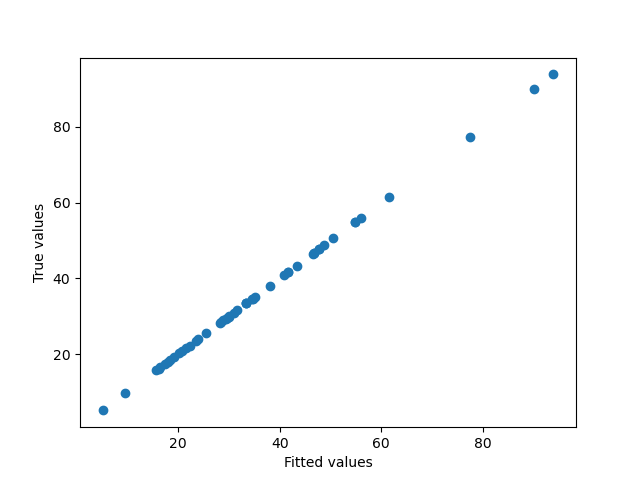
\includegraphics[width=0.65\textwidth]{../../../output/figures/Exploration/fit_utilization_JudgeID}
      \caption{True vs Fitted Values, Judge Model}
    \end{figure}

    \begin{table}[H]
      \centering
      % \small
      \caption{Judge Model}
      \begin{tabular}{rrr}
\toprule
 Iteration &  Beta P &  Beta T \\
\midrule
         0 &    0.15 &    6.48 \\
         1 &    0.07 &    3.12 \\
         2 &    0.07 &    3.12 \\
\bottomrule
\end{tabular}

    \end{table}

  \subsection{County Model}

    \begin{table}[H]
      \centering
      % \small
      \caption{County Model}
      \begin{center}
\begin{tabular}{lclc}
\toprule
\textbf{Dep. Variable:}    &        y         & \textbf{  R-squared (uncentered):}      &     0.995   \\
\textbf{Model:}            &       OLS        & \textbf{  Adj. R-squared (uncentered):} &     0.995   \\
\textbf{Method:}           &  Least Squares   & \textbf{  F-statistic:       }          &     4553.   \\
\textbf{Date:}             & Wed, 08 Sep 2021 & \textbf{  Prob (F-statistic):}          &  1.01e-51   \\
\textbf{Time:}             &     11:40:08     & \textbf{  Log-Likelihood:    }          &   -157.08   \\
\textbf{No. Observations:} &          46      & \textbf{  AIC:               }          &     318.2   \\
\textbf{Df Residuals:}     &          44      & \textbf{  BIC:               }          &     321.8   \\
\textbf{Df Model:}         &           2      & \textbf{                     }          &             \\
\bottomrule
\end{tabular}
\begin{tabular}{lcccccc}
               & \textbf{coef} & \textbf{std err} & \textbf{t} & \textbf{P$> |$t$|$} & \textbf{[0.025} & \textbf{0.975]}  \\
\midrule
\textbf{Plea}  &       0.1445  &        0.005     &    29.177  &         0.000        &        0.134    &        0.154     \\
\textbf{Trial} &       4.4126  &        0.324     &    13.619  &         0.000        &        3.760    &        5.066     \\
\bottomrule
\end{tabular}
\begin{tabular}{lclc}
\textbf{Omnibus:}       & 56.300 & \textbf{  Durbin-Watson:     } &    2.055  \\
\textbf{Prob(Omnibus):} &  0.000 & \textbf{  Jarque-Bera (JB):  } &  376.354  \\
\textbf{Skew:}          & -3.024 & \textbf{  Prob(JB):          } & 1.89e-82  \\
\textbf{Kurtosis:}      & 15.641 & \textbf{  Cond. No.          } &     149.  \\
\bottomrule
\end{tabular}
%\caption{OLS Regression Results}
\end{center}

    \end{table}

    \begin{figure}[H]
      \centering
      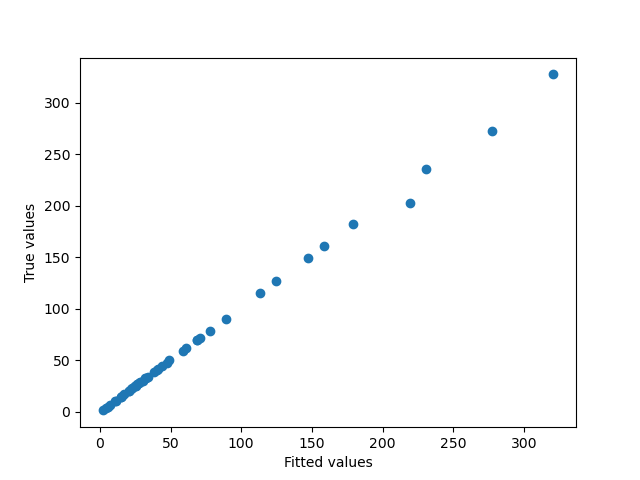
\includegraphics[width=0.65\textwidth]{../../../output/figures/Exploration/fit_min_County}
      \caption{True vs Fitted Values, Judge-County Model}
    \end{figure}

    \begin{table}[H]
      \centering
      % \small
      \caption{Judge Model}
      \begin{tabular}{rrr}
\toprule
 Iteration &  Beta P &  Beta T \\
\midrule
         0 &    0.15 &    3.61 \\
         1 &    0.14 &    3.67 \\
         2 &    0.14 &    3.65 \\
\bottomrule
\end{tabular}

    \end{table}

  \subsection{Judge-County Model}

    \begin{table}[H]
      \centering
      % \small
      \caption{County Model}
      \begin{center}
\begin{tabular}{lclc}
\toprule
\textbf{Dep. Variable:}    &        y         & \textbf{  R-squared (uncentered):}      &     0.986   \\
\textbf{Model:}            &       OLS        & \textbf{  Adj. R-squared (uncentered):} &     0.986   \\
\textbf{Method:}           &  Least Squares   & \textbf{  F-statistic:       }          &     9809.   \\
\textbf{Date:}             & Wed, 08 Sep 2021 & \textbf{  Prob (F-statistic):}          & 4.19e-257   \\
\textbf{Time:}             &     11:40:09     & \textbf{  Log-Likelihood:    }          &   -491.26   \\
\textbf{No. Observations:} &         278      & \textbf{  AIC:               }          &     986.5   \\
\textbf{Df Residuals:}     &         276      & \textbf{  BIC:               }          &     993.8   \\
\textbf{Df Model:}         &           2      & \textbf{                     }          &             \\
\bottomrule
\end{tabular}
\begin{tabular}{lcccccc}
               & \textbf{coef} & \textbf{std err} & \textbf{t} & \textbf{P$> |$t$|$} & \textbf{[0.025} & \textbf{0.975]}  \\
\midrule
\textbf{Plea}  &       0.0668  &        0.001     &    58.241  &         0.000        &        0.065    &        0.069     \\
\textbf{Trial} &       4.2463  &        0.058     &    72.973  &         0.000        &        4.132    &        4.361     \\
\bottomrule
\end{tabular}
\begin{tabular}{lclc}
\textbf{Omnibus:}       & 507.684 & \textbf{  Durbin-Watson:     } &     1.990   \\
\textbf{Prob(Omnibus):} &   0.000 & \textbf{  Jarque-Bera (JB):  } & 235811.290  \\
\textbf{Skew:}          & -10.399 & \textbf{  Prob(JB):          } &      0.00   \\
\textbf{Kurtosis:}      & 144.157 & \textbf{  Cond. No.          } &      61.2   \\
\bottomrule
\end{tabular}
%\caption{OLS Regression Results}
\end{center}

    \end{table}

    \begin{figure}[H]
      \centering
      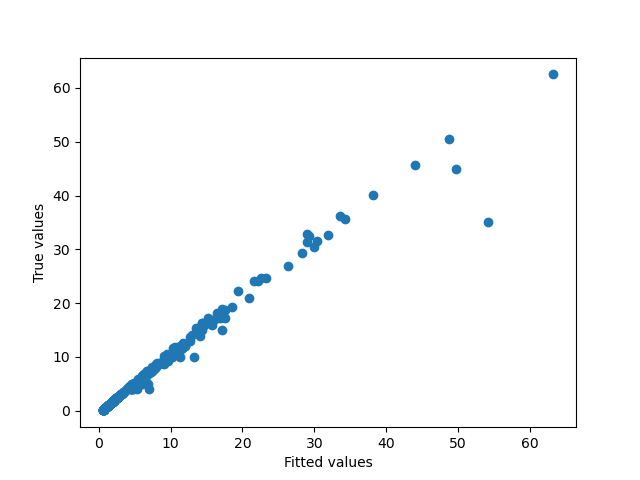
\includegraphics[width=0.65\textwidth]{../../../output/figures/Exploration/fit_min_JudgeIDCounty}
      \caption{True vs Fitted Values, Judge-County Model}
    \end{figure}

    \begin{table}[H]
      \centering
      % \small
      \caption{Judge-County Model}
      \begin{tabular}{rrr}
\toprule
 Iteration &  Beta P &  Beta T \\
\midrule
         0 &    0.10 &    4.19 \\
         1 &    0.08 &    4.11 \\
         2 &    0.07 &    4.09 \\
\bottomrule
\end{tabular}

    \end{table}

\section{Fixed Effects Model}
  We know from our exploratory analysis that there is large heterogeneity in activity amongst counties. Therefore, it is likely that the county that a judge happens to be in also significantly affects the number of pleas he is able to process. One way we could try to incorporate both judge and county idleness, would be to use
  a fixed effects model.  Here, the unit of observation would be a judge-county combination. For each judge county combination, $i$ with judge $j$ and county $c$, we could run the regression $\text{Days}_i = \alpha_j + \delta_c + \beta_p \text{Plea}_i + \beta_t \text{Trial}_i + \epsilon_i$. \textbf{Pros:} this would flexibly control for both judge and county fixed effects. \textbf{Cons:} We only have 248 observations of judge county combinations, and we would be trying to estimate around 96 parameters.

  \subsection{Model with Judge and County Fixed Effects}
    \begin{table}[H] \centering
      \caption{Fixed Effects Model}
    \begin{tabular}{@{\extracolsep{5pt}}lc}
    \\[-1.8ex]\hline
    \hline \\[-1.8ex]
     & \multicolumn{1}{c}{\textit{Dependent variable:}} \\
    \cline{2-2}
    \\[-1.8ex] & Days \\
    \hline \\[-1.8ex]
     Plea & 0.099$^{***}$ \\
      & (0.009) \\
      & \\
     Trial & 3.714$^{***}$ \\
      & (0.399) \\
      & \\
    \hline \\[-1.8ex]
    Observations & 278 \\
    R$^{2}$ & 0.801 \\
    Adjusted R$^{2}$ & 0.696 \\
    Residual Std. Error & 7.380 (df = 181) \\
    \hline
    \hline \\[-1.8ex]
    \textit{Note:}  & \multicolumn{1}{r}{$^{*}$p$<$0.1; $^{**}$p$<$0.05; $^{***}$p$<$0.01} \\
    \end{tabular}
    \end{table}

    \begin{figure}[H]
      \centering
      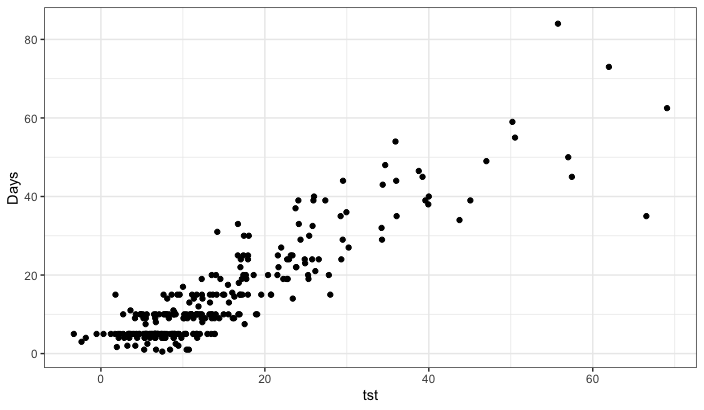
\includegraphics[width=0.65\textwidth]{../../../output/figures/Exploration/true_vs_fitted_fixed}
      \caption{True vs Fitted Values, fixed effects model}
    \end{figure}

  \subsection{Model with Judge Fixed Effects}
    Note, the unit of observation here, $i$, is the judge-county combination. The regression we are running here is:  $\text{Days}_i = \alpha_j + \beta_p \text{Plea}_i + \beta_t \text{Trial}_i + \epsilon_i$

    \begin{figure}[H]
      \centering
      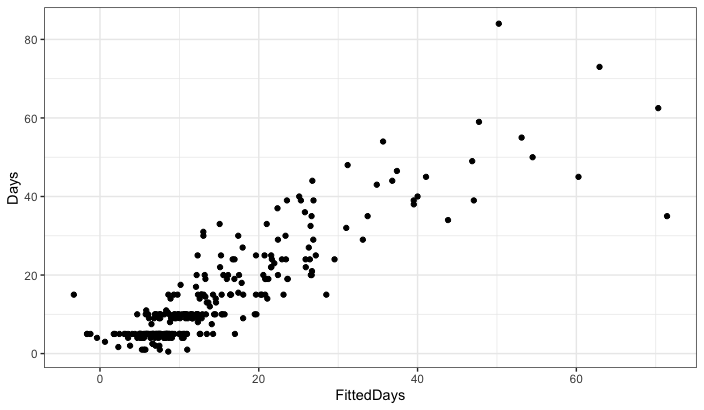
\includegraphics[width=0.65\textwidth]{../../../output/figures/Exploration/fit_fixed_JudgeID}
      \caption{True vs Fitted Values, fixed effects model}
    \end{figure}

    \begin{table}[H] \centering
      \caption{Model with Judge Fixed effects, table continues on next page}
      \small
      \begin{tabular}{@{\extracolsep{5pt}}lc}
      \\[-1.8ex]\hline
      \hline \\[-1.8ex]
       & \multicolumn{1}{c}{\textit{Dependent variable:}} \\
      \cline{2-2}
      \\[-1.8ex] & Days \\
      \hline \\[-1.8ex]
       Plea & 0.105$^{***}$ \\
        & (0.007) \\
        Trial & 3.861$^{***}$ \\
        & (0.349) \\
        Judge 1 & 15.166$^{***}$ \\
        & (3.192) \\
        Judge 10 & 5.090$^{**}$ \\
        & (2.532) \\
        Judge 11 & 10.027$^{**}$ \\
        & (4.280) \\
        Judge 12 & 7.506$^{**}$ \\
        & (2.907) \\
        Judge 13 & 7.795$^{***}$ \\
        & (2.697) \\
        Judge 14 & 6.221$^{**}$ \\
        & (2.901) \\
        Judge 15 & 4.168 \\
        & (2.681) \\
        Judge 16 & $-$5.497$^{*}$ \\
        & (2.857) \\
        Judge 17 & 7.804$^{**}$ \\
        & (3.573) \\
        Judge 18 & 9.869$^{***}$ \\
        & (3.243) \\
        Judge 19 & 4.191$^{*}$ \\
        & (2.256) \\
        Judge 2 & 9.071$^{***}$ \\
        & (3.232) \\
        Judge 20 & 3.862 \\
        & (3.544) \\
        Judge 21 & 5.074$^{**}$ \\
        & (2.509) \\
        Judge 22 & 6.544$^{**}$ \\
        & (3.230) \\
        Judge 23 & 8.460$^{**}$ \\
        & (3.552) \\
        Judge 24 & 2.276 \\
        & (3.787) \\
        Judge 25 & 4.645 \\
        & (2.956) \\
        Judge 26 & 5.215$^{*}$ \\
        & (2.711) \\
        Judge 27 & 5.405$^{*}$ \\
        & (3.180) \\
       \hline \\[-1.8ex]
      Observations & 278 \\
      R$^{2}$ & 0.897 \\
      Adjusted R$^{2}$ & 0.873 \\
      Residual Std. Error & 7.083 (df = 226) \\
      F Statistic & 37.788$^{***}$ (df = 52; 226) \\
      \hline
      \hline \\[-1.8ex]
      \textit{Note:}  & \multicolumn{1}{r}{$^{*}$p$<$0.1; $^{**}$p$<$0.05; $^{***}$p$<$0.01} \\
      \end{tabular}
    \end{table}

    \begin{table}[H] \centering
      \caption{Model with Judge Fixed effects, continued}
      \small
      \begin{tabular}{@{\extracolsep{5pt}}lc}
      \\[-1.8ex]\hline
      \hline \\[-1.8ex]
       & \multicolumn{1}{c}{\textit{Dependent variable:}} \\
      \cline{2-2}
      \\[-1.8ex] & Days \\
      \hline \\[-1.8ex]
        Judge 28 & 6.515$^{**}$ \\
        & (2.523) \\
        Judge 29 & 8.555$^{***}$ \\
        & (2.910) \\
        Judge 3 & 4.491 \\
        & (3.186) \\
        Judge 30 & 8.495$^{***}$ \\
        & (3.231) \\
        Judge 31 & 10.782$^{***}$ \\
        & (4.107) \\
        Judge 32 & 4.786 \\
        & (2.903) \\
        Judge 33 & 5.387$^{*}$ \\
        & (2.939) \\
        Judge 34 & 7.227$^{**}$ \\
        & (3.594) \\
        Judge 35 & 7.920$^{**}$ \\
        & (3.553) \\
        Judge 36 & 5.340$^{*}$ \\
        & (3.173) \\
        Judge 37 & 3.862 \\
        & (2.896) \\
        Judge 38 & 3.776 \\
        & (2.906) \\
        Judge 39 & 2.007 \\
        & (2.926) \\
        Judge 4 & 6.081$^{**}$ \\
        & (2.915) \\
        Judge 40 & 8.950 \\
        & (7.257) \\
        Judge 41 & 12.298$^{**}$ \\
        & (5.017) \\
        Judge 42 & 0.685 \\
        & (3.572) \\
        Judge 43 & 7.053$^{**}$ \\
        & (2.912) \\
        Judge 44 & 3.976 \\
        & (2.925) \\
        Judge 45 & 10.256$^{***}$ \\
        & (2.898) \\
        Judge 46 & 0.315 \\
        & (2.716) \\
        Judge 47 & 10.001$^{***}$ \\
        & (3.601) \\
        Judge 48 & 6.506$^{**}$ \\
        & (2.913) \\
        Judge 49 & 16.034$^{***}$ \\
        & (3.203) \\
        Judge 5 & 2.240 \\
        & (3.632) \\
        Judge 50 & 6.510$^{**}$ \\
        & (2.724) \\
        Judge 6 & 3.219 \\
        & (3.640) \\
        Judge 7 & 5.911$^{**}$ \\
        & (2.794) \\
        Judge 8 & 2.905 \\
        & (2.369) \\
        Judge 9 & 6.692$^{***}$ \\
        & (2.526) \\
       \hline \\[-1.8ex]
      Observations & 278 \\
      R$^{2}$ & 0.897 \\
      Adjusted R$^{2}$ & 0.873 \\
      Residual Std. Error & 7.083 (df = 226) \\
      F Statistic & 37.788$^{***}$ (df = 52; 226) \\
      \hline
      \hline \\[-1.8ex]
      \textit{Note:}  & \multicolumn{1}{r}{$^{*}$p$<$0.1; $^{**}$p$<$0.05; $^{***}$p$<$0.01} \\
      \end{tabular}
    \end{table}

\end{document}
